\documentclass[12pt,a4paper]{thesis}
\usepackage[latin1]{inputenc}
\usepackage{amsmath}
\usepackage{amsfonts}
\usepackage{amssymb}
\usepackage{graphicx}
\usepackage[doublespacing]{setspace}
\usepackage[authoryear]{natbib}
\usepackage{url}
\begin{document}

\title{Spatial Interaction Network Simulation Methods for Ancient Settlement Distributions in Central Italy}

\maketitle

\tableofcontents

\chapter{Introduction}
\section{General Overview}

\paragraph{}
Human Landscapes are created by the necessary struggle of people to meet their social and economic needs.  Eckbo states, "Historically, these objectives have run a gamut from utility through increasing convenience, comfort, and luxury to the more conscious and ostentatious display of wealth and power" \citeyearpar[p. 8]{Eckbo69}. Thus, as societies have settled and developed urban communities, human culture intensified, which in turn magnified the relationship between the people and the earth. The result is that the landscape is created by human decisions whether or not it was their intent to do so \citetext{\citealp[3-8]{Eckbo69}; \citealp[161]{AnsWilSch01}}. These decisions result in connections between people, places, and groups, producing a network of spatial interactions. More specifically, network science, which is the study of links and nodes on a graph and the attributes that arise from their interconnectedness, provides methods for visualizing and investigating settlement structures throughout the landscape. Networks allow for an environment in which many individual actors or settlements interact with each other simultaneously, creating a summation of those influences at each node. They also have the ability to represent various levels of structure \cite[9-10]{KnoKuk92}. Together these characteristics provide the ability to take static components and weave them together to more closely look at how a system that was truly dynamic in nature would have evolved.

\paragraph{}
Space is, and has always been, a pervasive  element in the daily routine of humans which can be studied through a range of forms, from symbolic manifestations to more physical representations \cite[p. 282]{Harvey06}. Naturally any study focused on the development of humanity is geographic by nature since, as a species, we have proliferated at all scales. These two points extend  to research on the distribution of excavated remains, features amongst remains, and the examination of spatial interaction between them. As a result, it is sensible to apply a geographer's toolbox to certain questions within the archaeology domain \cite[p. 39-42]{Kantner08}

\paragraph{}
Yu-Fi Tuan \citeyear{Tuan76}, writes, "If history is a pillar of the humanities then historical geography ought to be the pillar of humanistic geography"(272). Following this line of thinking, archaeology and humanistic geography can be thought of as overlapping, and thus sharing a common goal of building a history of humans. Tuan also writes, "The vivid depiction of a region is perhaps humanistic geography's highest achievement" (273). As such, it can be argued that through spatial analysis we will enrich our perception of a region and therefore help answer broader questions about how a place becomes defined through the larger landscape within which it exists (274).

\paragraph{} 
The purpose of this research is to explore the spatial distribution of early Etruscan states within a geographic network structure in order to shed light on how space conditioned their development  and then subsequently influenced how these sites interacted with each other. Specifically, this research will focus on how these spatial effects  pertain to the site known as Poggio Civitate (Murlo), which is located approximately 25km southeast of Siena, Italy. By considering the entire region of ancient Etruria, which coincides heavily with the modern Italian province of Tuscany, it will be possible to examine Poggio Civitate's individual characteristics as well as its relationship to other settlements within a cohesive Etruscan society. It is hoped that new evidence will be contributed towards existing theories which seek to explain the nature of this wealthy settlement which was abruptly destroyed and has henceforth remained uninhabited.

\paragraph{}
Quantitative modeling will be embraced as the analytical framework within which to carry out the proposed spatial 
analysis. Large multi-dimensional datasets quickly become complicated and conceptually difficult to manage. Models become a necessity to mitigate these complexities. They also act as a tool to develop hypotheses since the models can be parameterized in such a way to test existing and new theories. By employing a common language they increase dissemination and communication within and between fields \citep{Wyl09}. Quantitative modeling's merits within archaeology are summarized below by \citep{ERK12}:

    
\begin{quote}
        "Despite our best attempts at deducing relationships from the artefacts found at them [sites], there is often little direct information about how sites interact. Quantitative modelling provides one response to this challenge. Good quantitative modelling can be insensitive to poor data, make assumptions and biases clear and debatable, and can allow us to provide possible answers to questions that could not be asked any other way. In the best case, such answers can be checked later from the archaeological record."(1)
\end{quote}

\paragraph{}
Three conceptually unique techniques will be employed in order to simulate relative spatial interactions amongst the sites in the study area: an agent-based model, a radiation analogy model, and a Hamiltonian gravitational model. As a consequence, each model provides varying interpretations of spatial interaction by approaching the problem from 3 different perspectives. A multitude of models offers the ability to compare and contrast different nuances of a phenomenon using the same spatial inputs. Furthermore, different representations that yield varying yet similar results will provide assurance that we are indeed capturing the intended actions.
Subsequent chapters will elaborate on the concepts presented here. Chapter two will begin with a brief history of the Etruscans  and how Poggio Civitate fits into that narrative. It will then introduce the concept of spatial interaction theory and spatial interaction modeling, followed by a review of spatial interaction studies within the field of archaeology. A final product of Chapter two will be the selection of the three models that will be employed in this research.  Next, Chapter three will provide an explicit statement of the research goals and hypotheses that pertain to this research. Chapter four can be broken into three sections; the first will establish the input data that will be used for all three models while the second will provide in-depth description of how each model will be used to simulate networks, and, finally, the third section will establish the appropriate metrics to analyze the networks . The resulting networks and their properties will be reported in Chapter 5. Finally, the discussions and conclusions (Chapter Six) will provide a holistic summary of the research overall, a comparison of the three models, the implications each has regarding specific research questions, and suggestions for future research.

\chapter{Literature Review}
\section{History of the Etruscans and Poggio Civitate}

\paragraph{}
Etruria generally refers to the society that dwelt in ancient Italy from the pre-historic era through to the flourishing of the Roman civilization. Indeed there is much evidence that Etruscan culture was adopted by the Romans and that  these two cultures co-existed before the expansion of the Romans and subsequent decline of the Etruscans \cite[30-32, 56-60]{Scu80}. The height of Etruscan culture included complex cities, naval prowess, and intricate craftsmanship. Evidence for occupation within Etruria exists as early as about 4-5 millenniums BCE though it is not until much later that  distinct Etruscan culture emerged. Four general time periods can be assigned in the assessment of Etruscan historical development: the Late Bronze Age (c. 1300-900 BCE), the Villanovan period (c. 900-750 BCE), the Orientalizing period (c. 750-580 BCE), and the Archaic/Classical period (c. 580-400 BCE). The geographic extent covered by the Etruscans (Figure \ref{fig:etruria}) is usually prescribed as Central Italy, though in reality their territory covered a wider area which encompassed modern Lazio, Tuscany, and parts of Umbria, Campania, Emilia and Veneto \cite[21, 38]{SpiSto92}. Their major cities were generally bound between the Arno river and Tiber river to the North and South and the Tyrrhenian Sea and the Apennine Mountains to the West and East. Within this context the landscape tended to vary so that there were several different environments inhabited by the Etruscans simultaneously. It is hypothesized that the earliest Etruscan populations were egalitarian and fairly spread throughout the landscape with no signs of urban nucleation \cite[44-46]{BarRas98}. 

\begin{figure}
\centering
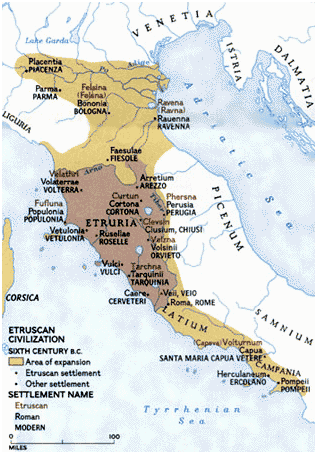
\includegraphics[width=0.7\linewidth]{../etruria}
\caption[Map of Etruscan Territory]{Map of Etruscan Territory}
\label{fig:etruria}
\end{figure}


\paragraph{}
As early as the 4th millennium B.C.E in Etruria, however, evidence shows that control over the production, distribution and consumption of resources was an important deciding factor in an individual's rank amongst his neighbors. Though there were few social divisions within these early societies, this practice of resource control was the basis for economic, political, and social competition which was the persistent driving force behind the process of their expansion. By the Late Bronze Age (1300-900 BCE) there was already significant intensification which lead to a shift from a landscape of only hamlets and farms to one that included, along with these, proto-urban villages. In this time period there was growth in the population with the appearance of new settlements, mostly on naturally defensible sites, valleys, and by major waterways. Expanded  territorial control fueled an increase in larger residences, hierarchical rankings, and economic activity with emphasis on animal secondary products, limited production of metals, and extensions of land use. While this time period still had a healthy population of inhabitants throughout the country it certainly marks the beginning of the process of nucleation and the formation of chiefdoms (44-59).

\paragraph{}  
Characterized by a dramatic increase in the process of nucleation, the Villanovan period (900-750 BCE), shows signs of further societal development.  Settlement numbers shrink considerably though those that prevail increase in population, size, and influence. Production and use of metals, especially iron, became indicators of wealth with much of the metals being obtained from key sources such as the Colline Metallifere, which translates to "Metal-bearing hills", or from the Tulfa Mountains \cite[75-77]{SpiSto92}. This is also the time period in which the first concrete evidence is recoded for habitation on the archaeological site of Poggio Civitate (Murlo). Located approximately 25km southeast of the Tuscan city of Siena on the eastern edge of the Colline Metillefere, this site shows three distinct phases of occupation on the plateau, Piano del Tesoro, of the hill. The earliest phase of occupation, the Iron Age (Coincides with Villanovan phase), is indicated by sparse remnants characteristic of pre-urban villages (citation forthcoming).

\begin{figure}
\centering
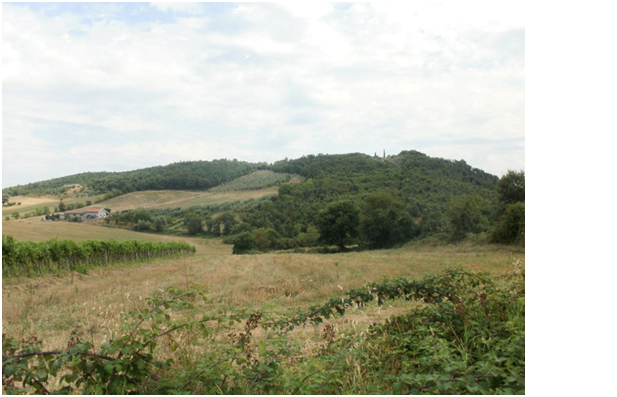
\includegraphics[width=0.7\linewidth]{../baseOfHill}
\caption{View of Poggio Civitate from the immediate periphery.}
\label{fig:baseOfHill}
\end{figure}

\paragraph{}
The later two phases of occupation differed in that they left behind significant archaeological remains of monumental architecture and are characterized by proto-urban traits such as craft specialization, social stratification, and increased consumption. The earlier of these two phases, starting in the 7th century BCE, consisted of three separate buildings (Figure \ref{fig:orientalizing}) each with a unique purpose: a tripartite building (three rooms) possibly for worship, a residence for an elite population, and a workshop for the manufacturing of bronze, bone, antler, ivory, food products, textiles, and architectural terracottas. A prolific burn layer in the soil stratigraphy along with unfired clay roofing tiles, which contained foot imprints, suggest that the site suffered from a sudden and fatal fire around 650 BCE. The plateau was subsequently scraped level and a new four-winged  complex (Figure \ref{fig:archaic}), approximately 60m in length each, was constructed (c. 600-580 BCE), which presumably incorporated all of the functions of the previous three buildings. Additional remains suggest the presence of watch towers and defensive walls that extended off of the main building. Unfortunately for the residents of the hilltop complex, it only survived a few decades before it was destroyed and abandoned between 550 and 535 BCE \cite[p. 35-45]{NieTuc01}

\begin{figure}
\centering
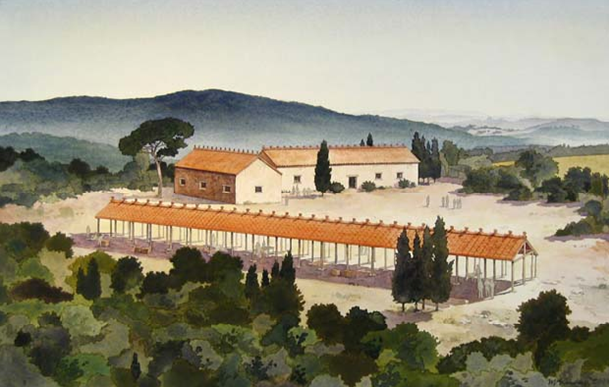
\includegraphics[width=0.7\linewidth]{../orientalizing}
\caption{Rendering of Orientalizing era (phase I) monumental architecture.}
\label{fig:orientalizing}
\end{figure}

\begin{figure}
\centering
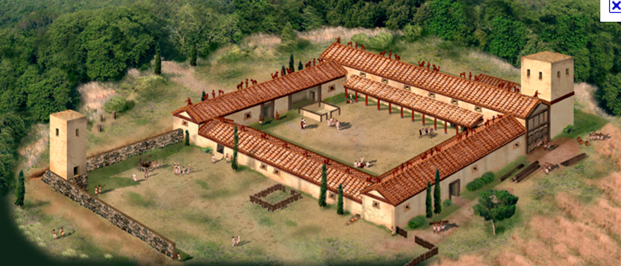
\includegraphics[width=0.7\linewidth]{../archaic}
\caption{Rendering of Archaic era (phase II) monumental architecture.}
\label{fig:archaic}
\end{figure}

\paragraph{}
While the exact reason for Poggio Civitate's eradication is unknown, the archaeological remains undeniably indicate that the occupants of the site commanded substantial authority.  The monumental architecture had rooftops adorned with captivating decorations (Figure \ref{fig:roof}) which would have been visible from afar and projected a message of social status to those at the site and within its periphery \citep{Tuc06,Odo13}. Additionally, the Archaic phase building featured a series of four recurring plaques displaying the lifestyle of an elite culture \cite[159]{Win09}. Due to a sudden destruction of the buildings, many items, normally considered portable, were left behind, including sets of elaborate bucchero cups, imported Greek vessels, large storage vessels, and hundreds of plates. This assemblage, which allows a glimpse into the society that dwelt on this hill, supports the theory that residents partook in banquets and feasts \cite[162-166]{BarRas98}. Material evidence signifies that those in control at Poggio Civitate likely dominated control over local natural resources and labor power. 

\begin{figure}
\centering
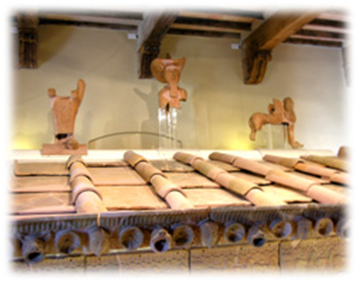
\includegraphics[width=0.7\linewidth]{../roof}
\caption{Rooftop decorations and statures.}
\label{fig:roof}
\end{figure}

\paragraph{}
Despite the status of the community at Poggio Civitate the site was not rebuilt after its destruction in the second half of the Sixth century BCE. In fact it was never reoccupied again and this seems to have been the intended goal of those responsible for the center's obliteration: as the walls were torn down the architectural terracottas were brought crashing to the ground. Some of the debris was then deliberately deposited in depressions throughout the site and covered with stone. The walls, along with soil and terracotta debris, were used to construct a mound, up to four meters high in some areas, along the perimeter of the plateau of Piano del Tesoro \citep{IEB94}. Additionally, roofing tiles were carried approximately 147.5m away from the Archaic phase building to intentionally seal a well that is speculated to have served a metal smelting industry or perhaps a residual community of Poggio Civitate \citep{TucBruHunTal10}. These actions maintain the theory that the destructors purposefully closed the hilltop site.

\paragraph{}
The permanent abandonment of the commanding hilltop of Poggio Civitate is surprising since modern civilization has proliferated on the crests of all other local hills. Many of these sites have in turn yielded archaeological remains from multiple eras \citep{Cam01}. It can be concluded that much of the landscape has been dotted with communities from ancient times until the present, except for Poggio Civitate.  After more than 40 years of excavations it is still unclear what forces caused residents to permanently vacate the hill's premises and why the hill was not resettled.

\paragraph{}
Everything that is known about Poggio Civitate, lacking formal reference in ancient texts, hails directly from the site's remains and the archaeologists who interpret them. Theories about why the settlement was destroyed or who the residents were must ultimately remain speculative. Modern literature produces a few prevailing, though vague, theories which attempt to answer questions about the origins and destruction of this elite civilization. 

\paragraph{}
Authors Barker and Rasmussen go as far as a general theory on the disappearance of Poggio Civitate. They explain that Murlo would have fallen into a category of medium-sized settlements that, due to their inland locations, were out of reach of the political authority of the larger cities. Though they would have initially developed autonomously, eventually these centers were abandoned or destroyed at a time when the major cities were growing in size and power. This is to say, simply, that these smaller centers were the 'losers' in the process of urbanization and expansion. The authors distilled their theory out of the fact that Etruscan cities likely controlled extensive land beyond their city limits \cite[p. 100,176]{BarRas98}. As any municipality grew in size they would have needed to destroy opposition and maintain a network of governance to ensure hegemony in their territory. Barker and Rasmussen do not develop their speculation any further but from their ideas it is easy to imagine Poggio Civitate as a rival settlement where the inhabitants were overthrown by enemies. Setti and Bonamici \citeyearpar{SetBon85} posit that the settlement of Chiusi was relatively late in the urbanization process showing its first signs of aristocracy only by the end of the 7th century BCE, and displaying typical behavior of Etruscan cities by the mid-6th century. They list military control of the countryside and abandoning of the small scattered communities as two such indicators of the development process, similar to imagined scenarios based on Barker and Rasmussen's theory. Setti and Bonamici proceed by stating that Murlo, located on the border between Chiusi's and Rusellae's territory, was the first of many (Dolciano Sarteano, Cetona) communities to be abandoned. She pegs the rise of the Chuisian King, Porsenna, and the expansionist policy that he initiated to the approximate date of Poggio Civitate's abandonment in 525 BCE (32-33). Due to Murlo's centrality between the major cities of Volterra, Arezzo, Chiusi, Roselle, and Vetulonia, and the evidence for its ritual status, Edlund-Berry \citeyearpar{IEB94} argued that the site might have operated as a neutral meeting place for a confederation of these cities, under divine protection, until the confederation was abolished when Chiusi changed its political affiliation to the Tarquin dynasty at the end of the sixth century BCE \cite[p. 176-177]{BarRas98}.

\paragraph{}	
These various theories attempt to answer questions pertaining to Murlo though ultimately they are unable to provide evidence beyond a casual narrative.  Generally, they develop their theories by looking to the remains of the site itself or to that of another site to explain the series of events that define Murlo without considering the space between them. Aspatial, and sometimes site-centric approaches to collecting corroborating evidence or deducing theories, while useful, can be at a serious disadvantage for researching processes that occur at several scales over a large territory. This research is aimed at developing a more rigorous methodology that includes site-centric information but also includes a regional setting to test hypotheses pertaining to Murlo. More specifically, spatial interaction models will be deployed to test how Murlo's spatial attributes such as size and location would have defined its role in relation to other sites within the entirety of the Etruscan society.  The connectivity networks that result from the models will help to depict the developing Etruscan landscape and subsequently alleviate the mysteries surrounding Poggio Civitate.


\section{Spatial Interaction Theory In Archaeology and Within Etruria}

\paragraph{}
Interaction within regions seems to enjoy popularity as a theory of a driver for growth within civilizations \citetext{\citealp[226]{Kow08}; \citealp[380]{Bin83}}. Colin Renfrew \citeyearpar{Ren75} provides one of the most complete theories of interaction, in the form of trade, as a driver for the development of early states.  In this archaeological context he identifies examples of territories in which neighbors are modular central places defined  by evenly spaced settlements at about a 1500km square area and a mean distance of 40km to neighbors, although this latter measure has been shown to range from 20km to 100km (14). While Renfrew credits trade as the mechanism behind the spatial interaction, he also discusses how these interactions rely on the interdependence of material and spiritual aspects of human culture and inevitably leads to communication and information flows as well (4-5, 24-25). His argument is that habitual exchange leads to central places since it requires organization and security and it implies some assumed criteria of value. He is careful to insist, however, that central places do not necessarily require civilization, but that they inevitably result in some form of interaction amongst those within the nucleated settlement (6-7). Ultimately, these central places provide a wealth of benefits in the form of market efficiency, as well as forums for solidarity and conflict resolution.  Competing centers result in more specialization that will further demand for the trade of goods between central places thus promoting greater interaction (9-10, 26-29).

\paragraph{}	
According to Renfrew, trade can be broken down into different categories,  including extra-regional trade, internal trade within a settlement's domain and trade between these domains within a region.  It is this last form of trade that Renfrew claims is the least studied despite the idea that its "effect must have been to produce and maintain the uniformity of culture or civilization as a whole" (18). He also states that "Civilization implies the development of a highly structured and differentiated society, with specialist production (craftsmen), a permanent controlling organization disposing of a significant proportion of produce (government), and a developed, explicit set of shared beliefs (cognitive structure), sometimes with large aggregations of population" (35). This suggests that those sites which have remains indicative of increasingly civilized characteristics would have likely participated in more inter-site trade amongst the larger central places. Similarly, Izzet cites increased encounters with 'others' as a driving factor in attitude changes towards ethnic identity. In this process, the differentiation of the self is an effect which takes place only after  discovering 'others' (2007, 210) . Physical growth and cultural development are therefore inextricably linked and, to a certain degree, controlled through the common process of interacting through space. 

\paragraph{}
It is difficult to differentiate between interaction and the growth of civilization. For example, population increases, which may have resulted from market benefits gained through trade and interaction, would have been likely to cause squabbles over territory. Tension amongst regions would initiate contact as well as competition which results in greater cultural development as well as further interaction (234). In contrast, the process of state emergence can be envisioned from the standpoint of external trade \citep{Pen11} using the Kipp-Schortmann model. This model holds that when a state society initiates contact with a chiefdom society, the elites of the latter, who will likely be sole recipients of the initial exchange, will experience an increase in power through the acquisition of new prestige goods. To maintain their authority over access to the new commodities the elites will resort to violating social norms which eventually erodes their legitimacy.  From the collapse of their power emerges the new organization of the state (181-183). Pena admits that his application of this model within Etruria produces pessimistic conclusions (196). Interestingly, he doesn't even consider internal trade as the mechanism that leads to the formation of states within Etruria. It is easy, however, to envisage this process occurring between social groups with differing ranks within a hierarchical structure without even incorporating external groups. If prestige is gained from trade goods that originate from farther away, more prestigious places then it is evident that distance played an important factor in the development of the involved societies. While it is still difficult to prove that this concept directly lead to more complex civilization it does nicely portray the importance on spatial contexts within Etruria which is able to provide a strong theoretical framework for measuring interactions amongst different groups. 

\section{Modern Transportation Geographic Theory}

\paragraph{}
Modern geographic theory pertaining to transportation studies is largely in agreement with the theories that have been developed within archaeology and are therefore helpful in providing a supporting theoretical framework for spatial interaction modeling. At the root of transportation theory lies the idea of complementarity which holds that different locations must have varying surpluses and deficits in order for the exchange of goods, ideas or people to occur (Comtois, Rodrigue, and Slack, 2006, 7). The ensuing interactions are further conditioned by environmental factors such as topography, hydrography, and climate. For example, transportation has historically followed paths along plains, valleys, and mountain passes while avoiding physical impediments. Similarly, available waterways, ports, access to natural resources and severe weather have been major considerations within transportation systems (8). What each of these factors have in common is that they incur a cost which must be considered against the benefits of carrying out the proposed transportation. Clearly, the spatial structure of the resulting transport network is a product of these environmental factors along with properties at each location which facilitate the creation of supply and demand and therefore affect the associated costs. In archaeology the decision process of whether or not to interact and subsequently travel from one site to another would have involved the same factors so that the derived spatial structure of an interaction network would be subject to the same constraints.    

\paragraph{}
	
The accessibility, or the measure of a site's ability to reach or be reached by another site, is a product of the established spatial structure. Distance, which is often measured by cost, is inversely proportional so that more accessible sites tend to be closer together, have less associated costs and are deemed more valuable. Agglomeration and specialization of activities is likely to take place at more valuable locations to reduce transportation costs and therefore further increase the value of a location. A location specializing in a commodity or activity may also drive segregation between itself and other locations as a side effect. In the process of transportation development, two forces are constantly in effect: concentration and dispersion. Coupled with the fact that transportation systems are subjected to the constraints of historical spatial structures it is apparent that these networks are highly dynamic yet they are constantly being conditioned (11-28). Typically the networks evolve to increase efficiency, decrease costs, and increase accessibility. Archaeological interaction networks would have been under similar influences making their development equally as dynamic. It is also therefore possible to assume that a proposed interaction network based on physical attributes should approach an approximate maximum efficiency and accessibility. Given the complexities within transportation geography and the overlap in theory with ancient interaction networks it seems appropriate to employ modern analytical methods within archaeological contexts.



\section{Spatial Interaction Theory and Modeling}

\paragraph{}
Spatial interaction encompasses an array of behaviors, such as communication or movement which occur over geographic space as a result of a decision process \citep[1]{FotOke89}. Its broad definition has allowed it to support a diversity of research within migration, shopping, recreation, commodity and capital flows, communication, transportation networks, and commuting (Haynes AND Fotheringham, 1984). In each application a trade-off is considered between the benefits accrued through interaction versus the costs necessary to traverse space to carry out the interaction. By encoding spatial interaction into a mathematical model it is possible to explain an observed phenomena or to use observed data in order to make predictions about the future or alternative scenarios \citep[2]{FotOke89}. This is particularly useful in circumstances where the number of locations under consideration or the factors involved in the decision-making process are large. Typically the interaction can be summarized by a matrix in which each row, $i$,  represents a possible origin and each column, $j$, represents a possible destination. As a result the interaction between any two locations can be described by flow $ij$ and the total interaction in or out of a site can be found by summing a row or column.    
	
\paragraph{}
Earliest spatial interaction models were developed using an analogy to gravitational forces from the field of physics (Roy AND Thill, 2004, 2). The Newtonian gravity model is relatively simple:\\
				\begin{equation}
				T_{ij} = \frac{k(P_{i}*P_{j})}{D_{ij}}
				\label{eq:simpleGrav}
				\end{equation}
				
where $T_{ij}$ denotes the aggregate flow between origin $i$ and destination $j$, $P_{i}$ and $P_{j}$ represent the size, population, or density of the origin and destination, and $D_{ij}$ is the physical separation between these two locations. It is apparent that given fixed values of $P_{i}$ and $P_{j}$, as $D_{ij}$ is increased, the value for $T_{ij}$ will decrease, therefore accounting for the costs of overcoming further distances. Additional parameters were later added to reflect the relationship of spatial flows and explanatory variables \cite[216]{FotBruCha02} which allowed customization of the model for different applications.  The gravity model faced criticism for its lack of theoretical foundations despite the fact that it produced reasonably accurate estimates of spatial flows (217).  A more stable theoretical grounding was developed in the 1960's by the work of retail modelers and regional planners \cite[2]{RoyThi04}. In the 1970's Wilson introduced a new framework for interaction modeling which relied on maximizing the entropy of the flow system. An aggregate flow between two locations is considered a macro state which can be satisfied by various micro states. The fundamental principle in entropy-maximizing models is that the most likely macro state is one which can be described by the highest number of micro states \cite[17-19]{FotBruCha02}. Adding in constraints allows for the derivations of a family of models in which information about origins, destinations, or both can be added to the model before solving for the most likely state \cite[4]{Wil10}. Despite the analytical gains of the maximum entropy models, criticisms arose due to the fact that it was still based on a physical analogy and that many of the applications lacked a behavioral interpretation \citep{Oke04}.

\paragraph{}	
Consequently, more contemporary efforts in the development of spatial interaction modeling has been to derive models based on spatial information processing. Fotheringham \citeyearpar{Fot83} developed the competing destinations model to accommodate the fact that during the decision-making process an individual will be faced with a unique spatial distribution of alternative locations for every destination under consideration. The competing destinations model incorporates the fact that individuals do not always consider every other location. The attributes of each alternative can contribute to how and whether or not an individual considers it at all. As a result, it is entirely possible for decisions to be made that do not reflect maximum utility since they may not even evaluate every possible choice. More recently, Simini, Gonzalez, Maritan, and Barabasi \citeyearpar{Bar12} present the radiation model as an entirely new framework which deviates from the gravity law concept which has been at the core of most previous models. The authors assert that their model overcomes no fewer than six known limitations of some previous gravity law models, most notably of all is that the model is parameter free and therefore requires no previous flow data for calibration. They also claim that their model permits a lack of interaction to have a priority over benefits gained in interacting. For  each possible origin and destination pair, flows are predicted by comparing the benefits of interacting with one proposed destination to the benefits of interacting with each other site within a radius from the origin equal to the distance from the origin to the proposed destination. Formally, these flows are given by the following,
			
				\begin{equation}
				T_{ij} = T_{i}\frac{(M_{i}*N_{j})}{(M_{i}+S_{ij})(M_{i}+N_{j}+S_{ij})}
				\label{eq:originalRad}
				\end{equation}
				
where $T_{ij}$ represents the flow prediction, $M_{i}$ and $N_{j}$ are density measures (e.g. population or size of a settlement) of the origin and destination respectively, $S_{ij}$ is the total density of all other alternative locations, and $T_{i}$ is a scaling factor that represents a proportion of the total number of commuters starting at a location which serves to ensure that commuter flows are not larger than the origin population.  Thus the model depends not directly on the distance variable but rather the aggregate benefits (e.g. population of a city) available at all other alternative choices between the origin and destination lending itself to the analogy of radiation and absorption processes (1-2). 

\paragraph{}	
Performance of the radiation model's over the simple gravity model in a wide range of applications and scenarios (hourly mobility, daily commuting, yearly migrations) has proven to be superior (Cite this from article). Therefore, given the simplicity of the radiation model and its proposed gains in analytical accuracy, it will be chosen as one of the three models proposed for this research. In the context of ancient spatial interaction $M_{i}$ and $N_{j}$ will be given by a proxy for population (e.g. urban area) which will provide a relative measure of populations throughout the study region. At present, there is no known research in which this model has been employed in the field of archaeology, which will provide an interesting comparison to past work that is founded upon the gravity law and distance decay.

\section{Spatial Interaction Modeling in Classical Archaeology}

\paragraph{}	
Renfrew and Level's XTENT model \citeyearpar{RenLev79} was an attempt to model the effects of space within an archaeological region using a stronger theoretical framework. The model, which is based upon Renfrew's previously discussed (section 2.2)  theory of trade and statehood, was designed to divide territory between respective central places and is defined by six  axioms (145-146):

	
\begin{enumerate}
\item The human social group is defined by the habitual association of persons with a territory
\item Human organization is segmentary in nature: human spatial organization is therefore cellular and modular.
\item Basic social groups do not exist in isolation, but affiliate together into larger groups, meeting together at periodic intervals. 
\item Human society is often hierarchical in nature: Human spatial organization is therefore 	stratified.
\item The effective polity, the highest order of social unit, may be identified by the scale and 	distribution of central places.
\item Special interactions between polities undoubtedly take place, creating uniformities in 	artifact distribution: Such uniformities in themselves do not document societies or people.
\end{enumerate}

\paragraph{}
Following these lines of thought, we can conclude that a) within social groups people will periodically interact giving rise to meeting places, b) human societies are often hierarchical  which necessarily implies a spatial patterning, and c) between these social groups or polities there is interaction. They are sure to note that the distribution of artifacts due to these interactions, which would become more uniform with increased  exchange, would be less indicative of individual societies. This can be interpreted as warning against the perils of using objects as a proxy for populations and their interactions in certain contexts as opposed to geographic features such as urban extent. The authors admit that their theory gives rise to their own version of Central Place Theory though they maintain that it is different than Christaller's Central Place Theory of economic man (146). Ultimately, his model describes hierarchy through competition rather than evaluating how space mediated interaction within settlement networks. For this reason, the model will not be used in this research which seeks to directly compare relative spatial interaction; however, Stoddard and Redhouse's \citeyearpar{StoRed11} extension of the XTENT model to Etruria (Figure \ref{fig:stoddard}) provides insight into territorial dynamics of the region under inspection. They conclude that Poggio Civitate would have initially existed as an autonomous entity outside the of reach of larger settlements. Eventual expansion and competition resulted in its absorption (168-169), strongly agreeing with the arguments previously explained (section 2.1). Their interpretations are useful for the comparison of models results presented in later sections of this research. 

\begin{figure}
\centering
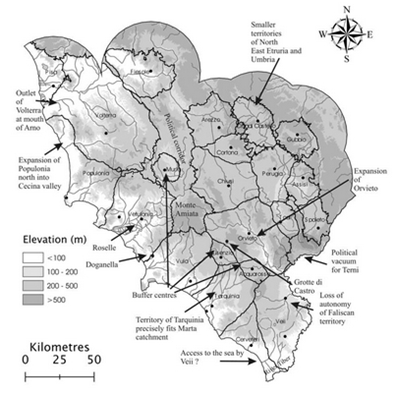
\includegraphics[width=0.7\linewidth]{../stoddard}
\caption{Results from the XTENT model for Etrura.}
\label{fig:stoddard}
\end{figure}

\paragraph{}
A simple model which has been employed in archaeology \citep{Bro00} for measuring connectivity is proximal point analysis (PPA). In PPA each site is connected to its $K$ nearest neighbors (constant value set by user) so that distance is not considered in the decision making process. In contrast, a maximum distance network (MDN) considers two sites connected if the distance between them is less than model parameter D, (constant value set by the user). Both models are inherently prohibitive, MDN's in that any site beyond the set distance is eliminated from the network and PPA in that a site may only maintain a limited number of links \cite[5-10]{ERK12}. One defining limitation of PPA approach is that all sites must participate thus forcing even the farthest sites to connect somewhere despite being potentially isolated. In a sense, both of these models are unrealistic because they only account for a limited set of scenarios. It is possible that sites close in proximity never visited each other due to resource sufficiency or  that communities located miles away still benefited from interaction regardless of distance and as a result made long journeys. Additionally, these simple models do not designate flow directions for the links; either two sites are simply connected or they are not which excludes the option for non-reciprocal relationships. The simplicity of these models makes them easy to apply but leaves many open questions during analysis.

\paragraph{}	
Gravity models were  adopted by David Clarke, a prominent spatial theorist within archaeology, who was a proponent of quantitative methods in the late 1960's and 1970's. In Analytical Archaeology he took a systemic and model approach to explain patterns in culture, technology, and the environment \citep{Cla68} and later in Spatial Archaeology \citep{Cla77}  he tackled issues of scale and space directly along with several additional authors who examined settlement structures, land use patterns and simulated the spread of settlements. This type of work was subjected  to the typical critiques of early quantitative methods. It was believed that  they over looked true social theory and that the anthropological neutrality claimed by these methods was actually biased towards the scientists employing them \cite[72]{Hod03}.

\paragraph{}
Building on previous work with gravity models Rhil and Wilson \citeyearpar{RihWil91} employ maximum entropy principles to simulate settlement patterns in Geometric mainland Greece. They ask the question, "Did location vis-a-vis other settlements have a significant effect on their affiliation and union?" (61). They argue that it is sufficient to use 'as the crow flies' straight lines despite lacking a true representation of Greece's rugged terrain because this information would have been incorporated in the dataset through settlements pre-determined locations and density. While they claim this assumption yields effective results it ignores the fact that settlement location selection and travel preferences constitute two different actions. A site may have been initially established for defense or proximity to resources without consideration or even any knowledge of many other site locations. Another important detail in Rhil and Wilson's model is that all sites start off with the same size and importance due to what they call the "egalitarian hypothesis" and these attributes are then predicted as part of the model. Validation is therefore possible between the model results and the attributes measured from the archaeological record. Two additional parameters, the benefits of concentrated resources and the difficulty of communication, enable the model to be fine tuned.   Their work offers an improvement on simple geographic models and elementary gravity models in archaeology by adding constraints and parameters, though it is not without flaws.  One limitation is that the model inherently creates networks that are 'supply side'. This means that larger cities attract the interactions of the nearest smaller sites, never allowing small sites to connect with each other. In effect, you get a network reminiscent of a star pattern (Figure \ref{fig:rhilWilson}) which is helpful for identifying key nodes but still may not represent a realistic network. Their gravity model also lacks the ability to capture the feedback effects of interactions and site size on each other \cite[10]{KnaEvaRiv08}.

\begin{figure}
\centering
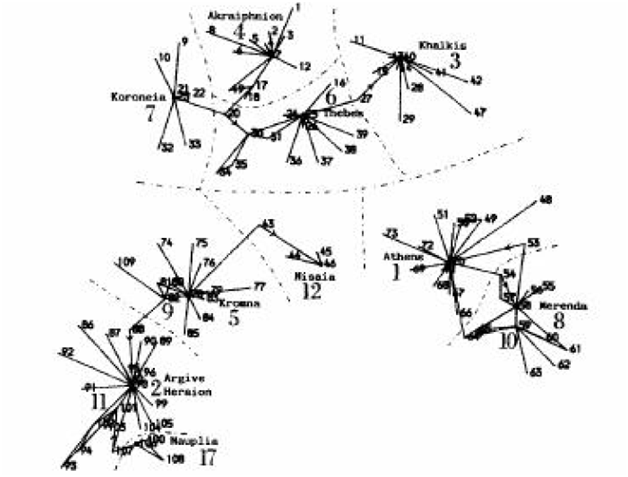
\includegraphics[width=0.7\linewidth]{../rhilWilson}
\caption{Results from Rhil and Wilson's maximum entropy gravity model.}
\label{fig:rhilWilson}
\end{figure}

\paragraph{}
Ariadne, the model developed by Evans et al., is a type of gravity model that has improved upon the work of Rhil and Wilson. They employ a 'Hamiltonian' energy function, H, consisting of four terms, which takes the form,
			\begin{equation}
			H = -kR - \lambda E + jP + \mu T
			\label{eq:simpleHam}
			\end{equation}  
where $R$ is the benefits of exploiting local resources, $E$ is the benefits of maintaining links, $P$ is the cost of supporting local populations and $T$ is the cost of maintaining links. Each term has a parameter which controls the effect it has within the model. Expanding the terms give $H$ the following form,
			\begin{equation}
			H = -k\sum_{i}S_{i}v_{i}(1-v_{i}) - \lambda\sum_{i,j}V(\frac{d_{ij}}{D})\cdot(S_{i}v_{i})\cdot e_{ij}\cdot (S_{j}e_{j}) + j\sum_{i}S_{i}v_{i} + \mu\sum_{i,j}S_{i}v_{i}e_{ij}
			\label{eq:expandedHam}
			\end{equation}

where $S_{i}$ is the given size of a site, $v_{i}$ and $e_{ij}$ are outputs of the model representative of the weight of each settlement and interaction link in the network, and $V(\frac{d_{ij}}{D})$ provides a gravity function based on the distance between two nodes ($d_{ij}$) and an average maximum journey length ($D$). $H$ provides a tool for balancing the cost and benefits of both 'supply' and 'demand' between site interactions. Using optimization techniques a minimum value is obtained for $H$ and the model output values ($v_{i}$ and $e_{ij}$) can be read off and visualized as a network (10-24). 

\paragraph{}
The additional output of interaction 'strength' ($e_{ij}$) makes it possible to create a network in which all nodes participate yet closer sites will have strong links and farther sites will have weaker ones. It is also feasible that some sites may choose not to interact because their costs outweigh the benefits. Unlike Rhil and Wilson, smaller neighbors are free to interact with each other rather than being limited to the hierarchical 'star' pattern. Ariadne is also superior because it incorporates "course-graining", the assumption that the whole is the sum of the parts, meaning that one value can be used to represent the exchange departing or arriving from multiple sites if they exist within a very close proximity. In archaeology this is crucial in supporting sometimes incomplete and ambiguous records for local regions. An important feature of the Ariadne model is that it is stochastic rather than deterministic. Each model run yields slightly different results which approach some optimal solution therefore mimicking short-term fluctuations within the system. A comparison of multiple runs allows the isolation of a most likely optimal solution \citep[12]{ERK12}. Due to Ariadne's abundance of advantages and ability to produce the most realistic settlement networks, it will be selected as the second model to simulate network interactions in central Italy. Ariadne's later deployment to investigate the effects of the destruction of a central node in the Greek maritime network as a result of the volcanic eruption of Thera \citep{KnaRivEva11} is directly comparable to the study of Poggio Civitate and its disappearance. Analysis in this research will therefore draw heavily from the methodology of Evans, Knappet, and Rivers.
	
\paragraph{}
Model three, inspired by the TravellerSim model, introduces an entirely new modeling framework into this research while still building off the work of by Rhil and Wilson. Graham and Steiner \citeyearpar{GraSte08} propose a method for observing the emergence of territories from the perspective of the individual. The general motivation for this agent-based approach is that it is not truly possible to know the exact relationship between sub-systems within a larger system. Instead we can assign very simple rules to individuals and then let them interact, thus developing the more complex relationships observed at the macro level. TravellerSim is built upon the same assumptions put forth by Rhil and Wilson \citep[64, 71]{RihWil91}, except spatial decisions are now limited to a local vision (approximately 20km from the settlement the agent is currently at). Each round, the agents consider 3 settlements within their vision and then choose to travel to the most 'attractive' destination. Attractiveness is calculated using a localized version of Rhil and Wilson's equation:

		\begin{equation}
	 	A = \frac{importance^{\alpha} * e^{-\beta D}}{visitors^{\alpha} * e^{-\beta D}}
		\label{eq:attractiveness}
		\end{equation}
	
where the importance is the current importance of a site, $\alpha$ is a parameter to represent the benefits from resources, $\beta$ is a parameter to represent the cost of communicating over space, and $D$ is the distance from the agent to the settlement whose attractiveness is being calculated. Settlements then update themselves based on each interaction they receive. 

\paragraph{}
In this manner the authors were able to successfully "grow" fuzzy territories and visualize the spread of influences over the region. Furthermore, by tracking the individual visits of the agents it is possible to visualize a weighted directed network similar to the Radiation model and Ariadne. In this respect, TravellerSim is not limited like Rhil and Wilson's model or the XTENT model despite their shared interest in hierarchy and territory. Overall, the bottom-up approach demonstrated in TravellerSim contributes a solid base on which to develop an interesting alternative to the more top-down concepts employed in the other two models selected for this research and will therefore be selected as the third model to study spatial interaction patterns within ancient Etruria. 

\chapter{Problem Statement and Hypothesis}

\paragraph{}
It is apparent from the literature (section 2.1) that there are two main theories which assume differing relationships over space. By defining the inherent inter-settlement associations, or lack thereof, that would have been present in each scenario we can develop tests to evaluate them. Our primary question, therefore, is "was Murlo an autonomous central place or did it feed into a larger hierarchy of settlements?"  we can then propose the following simplified theories from the literature on the nature of Poggio Civitate:
	
	\begin{enumerate}
	\item Murlo was a relatively autonomous settlement which enjoyed independence from the influence and authority of other central places despite its relatively smaller size.
	\item Murlo acted as central meeting place for the other Etruscan powers to meet in a neutral setting due to its central location to other settlements. 
	\end{enumerate}

\paragraph{}
To test these theories we need to embed Murlo into an interaction network with other contemporary sites. Theory one suggests that Murlo would have engaged in very little interaction given its location and size. More importantly, we must differentiate between incoming and outgoing interaction. For Murlo to remain autonomous we would expect relatively little incoming traffic since it was not subject to the influence of other settlements. Therefore, limited overall interaction will provide evidence for theory one though some outgoing interactions with minimal incoming interaction would still be considerably strong evidence. Conversely, theory two assumes strong interaction predictions amongst Murlo and its surrounding neighbors, especially in terms of incoming traffic. This is not to say that Murlo's neighbors would not have also interacted strongly with each other in their regular affairs. Rather, these interactions will be used as the base for a comparison to associations with Poggio Civitate.

\paragraph{}
Another objective of this research is to use a geographical approach to determine how the destruction of Poggio Civitate factored into the dynamics of the larger system. Unfortunately, the spatial distribution of settlements does not directly provide information on the demise of Murlo. Instead, we can use the quantitative models to simulate interaction networks with and without Murlo in order to answer the question, "How did the destruction of Poggio Civitate effect the strength and distribution of interaction throughout the wider region of Etruria?". If the network remains relatively unchanged it will count as evidence towards Murlo as an autonomous central place. Likewise, if we record large shifts in the network we can conclude that it is likely that Poggio Civitate was playing an important role in the wider region of Etruria and that its destruction may have been related to its favorable location. 

\chapter{Methodology}
\section{Data}

\paragraph{}
For all of the chosen models, the only necessary data is a selection of settlements, their geographic coordinates, a proxy for each site's population or size, and a measurement of distance between all pairs of sites. Considering Renfrew's warning against relying on artifact counts and the unavailability of population estimates, the urban extent of a site's archaeological remains will be used to represent its size. Settlements taken into consideration for this research are those used by Stoddart and Redhouse (2011) to test the Early State Module concept of Colin Renfew (1975). Under Renfrew's theory, the characteristics of early state societies included autonomous central places,  a uniform spacing of about 40km amongst neighbors, approximately 1500 square kilometers of territory per polis, and the region consisted of a cluster of about a dozen sites. Stoddart and Redhouse (2011) provide a list of 25 Etruscan settlements and their corresponding size estimates which co-existed in time period roughly from 900 to 600 BCE. Though their research shows that only a fraction of the sites ultimately meet the ESM standards using the XTENT model, we can nevertheless adopt their study sites for use in our spatial interaction models given that this research has no restriction to solely early states. Their data provides the best available starting point for spatial interaction modeling in this context because they have assembled site size estimates by drawing from various archaeological sources as well as personal experience when no estimation existed (166). Following Stoddart amd Redhouse, the sites, as presented in Figure \ref{fig:SiteData}, were all given spatial context via the Latitude and Longitude attributes from the Getty Thesaurus of Geographic Names Online with the exception of Bisenszio. Each site's name was queried in the on-line thesaurus, and if an entry existed for the ancient site as opposed to the modern one, then it was used. If only one entry existed (modern or ancient), then it was utilized. For Bisenzio, which was not listed in the thesaurus, coordinates were estimated visually using its known location via Google Earth.

\begin{figure}
\begin{tabular}{|c|c|c|c|c|}
\hline \textbf{Name} & \textbf{Number} & \textbf{Size} & \textbf{GettyLon} & \textbf{GettyLat} \\ 
\hline 	Veii	&	1	&	185	&	42.0333	&	12.4	\\
\hline 	Cerveteri	&	2	&	160	&	42	&	12.1	\\
\hline 	Vetulonia	&	3	&	100	&	42.85	&	10.9667	\\
\hline 	Populonia	&	4	&	150	&	42.9833	&	10.4833	\\
\hline 	Volterra	&	5	&	100	&	43.4	&	10.85	\\
\hline 	Chiusi	&	6	&	50	&	43.0167	&	11.95	\\
\hline 	Bisenzio	&	7	&	35	&	42.57	&	11.87	\\
\hline 	Acquarossa	&	8	&	30	&	42.4833	&	12.1333	\\
\hline 	Perugia	&	9	&	32	&	43.1333	&	12.3667	\\
\hline 	Gravisca	&	10	&	24	&	42.2	&	11.7167	\\
\hline 	Gubbio	&	11	&	20	&	43.35	&	12.5833	\\
\hline 	Assisi	&	12	&	20	&	43.0667	&	12.6167	\\
\hline 	Citta di Castello	&	13	&	20	&	43.45	&	12.2333	\\
\hline 	Tarquinia	&	14	&	150	&	42.25	&	11.75	\\
\hline 	Vulci	&	15	&	126	&	42.4167	&	11.5833	\\
\hline 	Roselle	&	16	&	40	&	42.8	&	11.1333	\\
\hline 	Murlo	&	17	&	10	&	43.15	&	11.3833	\\
\hline 	Pisa	&	18	&	20	&	43.7167	&	10.3833	\\
\hline 	Orvieto	&	19	&	85	&	42.7167	&	12.1167	\\
\hline 	Arezzo	&	20	&	32	&	43.4167	&	11.8833	\\
\hline 	Cortona	&	21	&	30	&	43.2667	&	11.9833	\\
\hline 	Civita Castellano	&	22	&	26	&	42.2833	&	12.4167	\\
\hline 	Fiesole	&	23	&	30	&	43.8	&	11.2833	\\
\hline 	Todi	&	24	&	20	&	42.7833	&	12.4	\\
\hline 	Spoleto	&	25	&	20	&	42.7333	&	12.7333	\\
\hline
\end{tabular} 
\caption{ Sites used in the study and their attributes.}
\label{fig:SiteData}
\end{figure}

 
\paragraph{}
It is important to note the possible boundary effects that might arise from this data set. While this list includes the significant settlements that existed throughout the time period of interest there would have undeniably been considerable interaction occurring between sites within the study region and those external to it, especially for those settlements close to the study region border. This is a problem that will arise at any scale and for any study region. Regardless, we must limit the boundaries in order to maintain conceptual simplicity as well as managing computing resources.  
	
\paragraph{}
Many  methods are available for obtaining inter-settlement distances. Straight line or 'as the crow flies' distance is the simplest measurement to employ since it requires no abstract concept of cost and can be easily computed using Euclidean distance calculations. It is obvious, however, that most network edges cannot be truly represented without incorporating the natural terrain. Bevan (forthcoming) reviews several alternate methods that have been deployed by archaeologists to integrate the landscape into distance calculations. Arguably an entire study could be completed solely on choosing a proper representation of travel times or costs over space. As a compromise, this research will leverage methods similar to those utilized by Stoddart and Redhouse (165) within the XTENT model whenever possible. This will promote consistency, incorporate the effects of the terrain, and  maintain simple and reproducible calculations. Ultimately the method employed here will differ since this research seeks to  incorporate the terrain by deriving likely paths between sites whereas Stoddart and Redhouse aimed to create cost distance rasters for the entire region.  

\paragraph{}	
Distances between sites will be reflective of the least accumulated cost path given the energy (Put units in here) necessary to traverse natural slopes within the terrain. To carry out this calculation an ASTER 30m resolution digital elevation model will be used to derive the slope of the terrain, which is an improvement in resolution over previous work \citep[165]{StoRed11}. The elevation DEM was clipped to a buffer of two times the average nearest neighbor distance (straight line) of the settlements and to the natural coast line of the Italian peninsula (167). A slope raster was then calculated with the clipped DEM as the input. Differing 'costs' to travel from one site to another were computed in terms of the energy expelled to navigate over varying slopes \citep{Min02} as proposed by Stoddard and Redhouse \citeyearpar{StoRed11}. Conclusions by Minetti Et al. include the cost of walking for both running and walking for slopes from -45 to 45 degrees. Since it is assumed that the distances between the sites is long enough that the average person could not completely run an entire trip the values for the cost of walking will be used. It should also be noted that for most slopes the cost of running is not much higher than walking and that the cost of running follows a similar increasing trend as the cost of walking. Additionally, since the slope data that is produced is represented solely with positive values (Since it really only depends then on the direction you are travelling) it is impossible to incorporate the entire range of results. Using a rough estimation, the costs as presented in table X (forthcoming- still need to do this) were assigned to different classes of slopes. The final output is a cost or friction raster which was used to derive the least accumulated cost paths in origin-destination matrix format (Etherington, 2011).(PROJECTion SITES?) These values are all considerably longer than the straight-line distances since they tend to closely gravitate towards areas with lesser slopes to find the routes which will require less energy to be exerted. Developing a distance measurement that is representative of a physical transportation network preserves the edge length units within the network which enhances the ease with which the model results can be interpreted. Additionally, a non-abstract measure of distance preserves the ability to be verified against both contemporary knowledge and future discoveries of ancient roads within the study region.



\section{Simulating Networks Using Spatial Interaction Models}


\paragraph{}


\section{Network Analysis Metrics}

\chapter{Results}
\section{Ariadne Model}
\section{Radiation Model}
\section{Agent-based Model}

\chapter{Discussion and Conclusions}
\section{Simulating Networks}
\section{Comparing and Contrasting the Models}
\section{Implications for Poggio Civitate}
\section{Final Conclusions}
\section{Further Work}

\bibliographystyle{apa-good}
\bibliography{bibfile}

\end{document}}